\documentclass [aspectratio=169]{beamer}
\usetheme{Boadilla}
\usepackage{textpos} % package for the positioning
\usepackage[]{graphicx}
\usepackage{graphicx}
\usepackage{float}
\usepackage{hyperref}
\usepackage{caption}
\usepackage{subcaption}
\usepackage{algorithm,algpseudocode}
\usepackage[export]{adjustbox}
\usepackage{tikz}
\usetikzlibrary{positioning}
\usetikzlibrary{arrows, shapes, decorations, automata, backgrounds, fit, petri, calc}
\setbeamertemplate{itemize items}[circle]
\setbeamertemplate{enumerate items}[circle]
\setbeamertemplate{itemize subitem}{$\triangleright$}


\newcommand*{\logofont}{\fontfamily{phv}\selectfont}
\definecolor{uoftblue}{RGB}{6,41,88} % official blue color for uoft

\vspace{1in}
\title[]{DoSS Summer Bootcamp Probability \\ Module 2}
\author[]{Ichiro Hashimoto}
\institute[]{University of Toronto}
\date{July 10, 2024}

% set color
\setbeamercolor{title in head/foot}{bg=white}
\setbeamercolor{author in head/foot}{bg=white}
\setbeamercolor{date in head/foot}{fg=uoftblue}
\setbeamercolor{date in head/foot}{bg=white}
\setbeamercolor{title}{fg=uoftblue}
\setbeamerfont{title}{series=\bfseries}
\setbeamercolor{frametitle}{fg=uoftblue}
\setbeamerfont{frametitle}{series=\bfseries}
\setbeamercolor*{item}{fg=uoftblue}
\setbeamercolor{block title}{bg=uoftblue}
\setbeamercolor{block title}{fg=white}
\setbeamercolor{block body}{bg=uoftblue!5!white}

% set logo at non-title pages
\logo{
\includegraphics[height=0.8cm]{logo_uoft.png}\vspace*{-.055\paperheight}\hspace*{.85\paperwidth}}

% set margin
\setbeamersize{text margin left=10mm,text margin right=10mm}

\newcommand{\mc}{\mathcal}

\begin{document}
{
\setbeamertemplate{logo}{}
\begin{frame}
    \vspace{0.5in}
    \titlepage
    \begin{textblock*}{4cm}(0.5cm,-7.5cm)
        
\includegraphics[width=4cm]{logo_uoft.png}
    \end{textblock*}
    \begin{textblock*}{8cm}(5.0cm,-7cm)
        \huge \color{uoftblue}{$\Bigr\rvert$ \hspace{0.15cm} \textbf{\logofont Statistical Sciences}}
    \end{textblock*}
\end{frame}
}

\begin{frame}{Recap}
Learnt in last module:\\
\vspace{0.1in}
   \begin{itemize}
        \item Measurable spaces
        \begin{itemize}
            \item Sample Space
            \item $\sigma$-algebra
        \end{itemize}
        \item Probability measures
              \begin{itemize}
            \item Measures on $\sigma$-field
            \item Basic results
        \end{itemize}
        \item Conditional probability
        \begin{itemize}
            \item Bayes’ rule
            \item Law of total probability
        \end{itemize}
    \end{itemize}
\end{frame}

\begin{frame}{Outline}
    \begin{itemize}
    	\item Independence of events % because we have not define random variables
    	\begin{itemize}
    	    \item Pairwise independence, mutual independence
    	    \item Conditional independence 
    	\end{itemize}
        \item Random variables
        \item Distribution functions
        \item Density functions and mass functions
        \item Independence of random variables
        %\begin{itemize}
         %   \item Convolutions
        %\end{itemize}
    \end{itemize}




\end{frame}

\begin{frame}{Independence of events}
\textbf{Recall the Bayes rule}:\\
$$P(A \mid B) = \dfrac{P(A\cap B)}{P(B)}, \quad P(B) > 0$$
\begin{itemize}
    \item<1-> What if $B$ does not change our belief about $A$?
    \item<2-> This means $P(A \mid B) = P(A)$.
    \item<3-> Equivalently, $P(A \cap B) = P(A)P(B)$.
\end{itemize}
\uncover<4->{
\begin{block}{Independence of two events}
Two events $A$ and $B$ are independent if $P(A \cap B) = P(A)P(B)$.
\end{block}
\textbf{Remark:}}
% A and B independent, then B and A independent
\vspace{0.2in}
\end{frame}


\begin{frame}{Independence of events}
\textbf{Consider more than 2 events:}\\
\uncover<1->{
    \begin{block}{Pairwise independence}
    We say that events $A_1, A_2, \cdots, A_n$ are pairwise independent if 
    $$P(A_i \cap A_j) = P(A_i) \cdot P(A_j), \quad \forall i \neq j $$
    \end{block}}
    \uncover<2->{
    \begin{block}{Mutual independence}
     We say that events $A_1, A_2, \cdots, A_n$ are mutually independent or independent if for all subsets $I \in \{1, 2, \cdots, n\}$
    $$P(\cap_{i \in I} A_i) = \prod_{i \in I} P(A_i) $$
    \end{block}}
    \uncover<3->{
    \textbf{Remark:}}\\ % for 2 events, these are equivalent, and mutual independence is stronger than pairwise independence
    \vspace{0.2in}
\end{frame}

\begin{frame}{Independence of events}
\textbf{Example:} % Here we need one example where mutual independence is not satisfied while pairwise independence is achieved
\begin{itemize}
    \item<1-> Toss two fair coins.;
    \item<1-> $A=\{$ First toss is head$\}$, $B =\{$ Second toss is head $\}$, $C = \{$ Outcomes are the same $\}$;
    \item<1-> $A = \{HH, HT\}, B = \{HH,TH\}, C = \{HH,TT\}$;
    \item<2-> $P(A \cap B) = P(A)P(B)$, $P(A \cap C) = P(A)P(C)$, $P(B \cap C) = P(B)P(C)$;
    \item<3-> $P(A\cap B\cap C) \neq P(A)P(B)P(C)$.
\end{itemize}
\vspace{0.1in}
\end{frame}

\begin{frame}{Independence of events}

\begin{block}{Conditional independence}
Two events $A$ and $B$ are conditionally independent given an event $C$ if
$$
P(A\cap B \mid C) = P(A \mid C)P(B \mid C).
$$
\end{block}
\uncover<2->{\textbf{Example:} \\
Previous example continued: 
\begin{itemize}
    \item $A = \{HH, HT\}, B = \{HH,TH\}, C = \{HH,TT\}$;
    \item ${P}(A\cap B \mid C) = ?$, ${P}(A \mid C){P}(B \mid C) = ?$
\end{itemize}
\vspace{0.1in}
}
\uncover<3->{
\textbf{Remark:}\\ 
Equivalent definition:
$$
{P}(A \mid B, C) = {P}(A \mid C).
$$}
\end{frame}


\begin{frame}{Random variables}
\textbf{Idea}:\\

Instead of focusing on each events themselves, sometimes we care more about functions of the outcomes.\\
\vspace{0.1in}
\uncover<2->{\textbf{Example}:\\
\begin{itemize}
    \item Toss a fair coin twice: $\{HH, HT, TH, TT\}$
    \item Care about the number of heads: $\{2, 1, 0\}$
\end{itemize}}
\uncover<3->{\begin{figure}
    \centering
    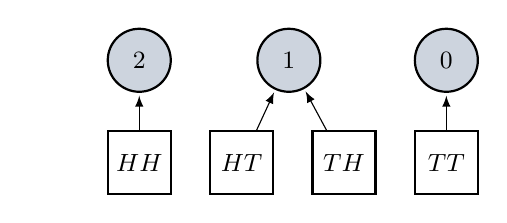
\begin{tikzpicture}[bend angle=45,>=latex, font=\small,scale=1, every node/.style={transform shape}]%
        
            \tikzstyle{obs} = [ circle, thick, draw = black!100, fill = uoftblue!20, minimum size = 0.8cm, inner sep = 0pt]
            \tikzstyle{lat} = [ circle, thick, draw = black!100, fill = red!0, minimum size =  0.8cm, inner sep = 0pt]
            \tikzstyle{par} = [ circle, thin, draw, fill = black!100, minimum size = 0.8, inner sep = 0pt]	
            \tikzstyle{det} = [ rectangle, thick, draw = black!100, fill = red!0, minimum size = 0.8cm, inner sep = 0pt]
            \tikzstyle{inv} = [ circle, thin, draw=white!100, fill = white!100, minimum size = 0.8cm, inner sep = 0pt]	
            \tikzstyle{every label} = [black!100]%
        %%
            \begin{scope}[node distance = 1.3cm and 1.3cm]%
                %% State variables
                \node (hr_tm2) {};
                \node [det] (hr_tm1) [ right of = hr_tm2]   {$HH$};
                \node [det] (hr_t) [ right of = hr_tm1]   {$HT$};
                \node [det] (hr_tp1) [ right of = hr_t] {$TH$};
                \node [det](hr_tp2) [ right of = hr_tp1]{$TT$};
                
                %% Outputs
                \node [obs] (x_tm1) [ above of = hr_tm1]   {$2$};
                \node [obs] (x_t) [ above of = hr_t, xshift = 0.6cm] {$1$};
                \node [obs] (x_tp1) [ above of = hr_tp2] {$0$};
                
                \draw[post] (hr_tm1) edge  (x_tm1);
                \draw[post] (hr_t) edge  (x_t);
                \draw[post] (hr_tp1) edge (x_t);
                \draw[post] (hr_tp2) edge (x_tp1);
            \end{scope}%
        \end{tikzpicture}%
    \caption{Mapping from the sample space to the numbers of heads}
    \label{fig:my_label}
\end{figure}}
    \vspace{0.1in}
\end{frame}

\begin{frame}{Random Variables}
\textbf{Example:}
\begin{itemize}
    \item Select twice from red and black ball with replacement: $\{RR, RB, BR, BB\}$
    \item Care about the number of red balls: $\{2, 1, 0\}$
\end{itemize}
\begin{figure}
    \centering
    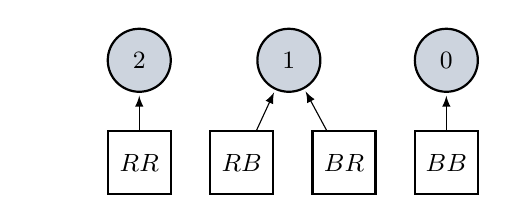
\begin{tikzpicture}[bend angle=45,>=latex, font=\small,scale=1, every node/.style={transform shape}]%
            \tikzstyle{obs} = [ circle, thick, draw = black!100, fill = uoftblue!20, minimum size = 0.8cm, inner sep = 0pt]
            \tikzstyle{lat} = [ circle, thick, draw = black!100, fill = red!0, minimum size =  0.8cm, inner sep = 0pt]
            \tikzstyle{par} = [ circle, thin, draw, fill = black!100, minimum size = 0.8, inner sep = 0pt]	
            \tikzstyle{det} = [ rectangle, thick, draw = black!100, fill = red!0, minimum size = 0.8cm, inner sep = 0pt]
            \tikzstyle{inv} = [ circle, thin, draw=white!100, fill = white!100, minimum size = 0.8cm, inner sep = 0pt]	
            \tikzstyle{every label} = [black!100]%
        %%
            \begin{scope}[node distance = 1.3cm and 1.3cm]%
                %% State variables
                \node (hr_tm2) {};
                \node [det] (hr_tm1) [ right of = hr_tm2]   {$RR$};
                \node [det] (hr_t) [ right of = hr_tm1]   {$RB$};
                \node [det] (hr_tp1) [ right of = hr_t] {$BR$};
                \node [det](hr_tp2) [ right of = hr_tp1]{$BB$};
                
                %% Outputs
                \node [obs] (x_tm1) [ above of = hr_tm1]   {$2$};
                \node [obs] (x_t) [ above of = hr_t, xshift = 0.6cm] {$1$};
                \node [obs] (x_tp1) [ above of = hr_tp2] {$0$};
                
                \draw[post] (hr_tm1) edge  (x_tm1);
                \draw[post] (hr_t) edge  (x_t);
                \draw[post] (hr_tp1) edge (x_t);
                \draw[post] (hr_tp2) edge (x_tp1);
            \end{scope}%
        \end{tikzpicture}%
    \caption{Mapping from the sample space to the numbers of red balls}
    \label{fig:my_label}
\end{figure}
\end{frame}


\begin{frame}{Random Variables}
    \textbf{Merits:}
    \begin{itemize}
        \item Mapping the complicated events on $\sigma$-field to some numbers on real line. 
        \item Simplify different events into the same structure
    \end{itemize}
    \uncover<2->{\begin{block}{Random Variables}
    Consider sample space $\Omega$ and the corresponding $\sigma$-field $\mc{F}$, for $X: \Omega \to \mathbb{R}$, if 
    $$A \in \mc{R}\quad (\text{Borel sets on } \mathbb{R}) \Rightarrow  X^{-1}(A) \in \mc{F},$$
    then we call $X$ as a random variable. \\
    Here $X^{-1}(A) = \{\omega: X(\omega) \in A\}$.\\
    We can also say $X$ is $\mc{F}$-measurable.
    \end{block}}
\end{frame}


\begin{frame}{Distribution functions}
\textbf{Probability measure $P(\cdot)$ on $\mc{F}$ can induce a measure $\mu(\cdot)$ on $\mc{R}$}:\\
\begin{block}{Probability measure on $\mc{R}$}
We can define a probability $\mu$ on $(R, \mc{R})$ as follows:\\
$$\forall A \in \mc{R}, \quad \mu(A):= P(X^{-1}(A)) = P(X \in A).$$
Then $\mu$ is a probability measure and it is called the distribution of $X$.
\end{block}
\vspace{0.1in}
\uncover<2->{
\textbf{Remark:}\\
Verify that $\mu$ is a probability measure.\\
\begin{itemize}
      \item $\mu(\mathbb{R}) = 1$.
    \item If $A_1, A_2, \cdots \in \mathcal{R}$ are disjoint, then $\mu(\cup_{i = 1}^{\infty} A_i) = \sum_{i = 1}^\infty \mu(A_i)$.
\end{itemize}}
\end{frame}

\begin{frame}{Distribution functions}
% need to explain why we only need to consider negative infinity to x?
\textbf{Consider the special set that belongs to $\mc{R}$, $(-\infty, x]$}:
\begin{block}{Cumulative Distribution Function}
The cumulative distribution function of random variable $X$ is defined as follows:
$$ 
F(x):= P(X \le x) = P(X^{-1}((-\infty,x])), \quad \forall x \in \mathbb{R}.
$$
\end{block}
\vspace{0.1in}
\uncover<2->{
\textbf{Properties of CDF:}\\
\begin{itemize}
    \item $\lim_{x \to \infty} F(x) = 1$, $\lim_{x \to -\infty} F(x) = 0$
    \item $F(\cdot)$ is non-decreasing
    \item $F(\cdot)$ is right-continuous % further explain this
    \item Let $F(x^{-}) = \lim_{y \nearrow x} F(y)$, then $F(x^{-}) = P(X < x)$
    \item $P(X = x) = F(x) - F(x^{-})$
\end{itemize}}
\end{frame}

\begin{frame}{Distribution functions}
    \textbf{Proofs of properties of CDF (first 2 properties):}\\
    \vspace{2.5in}
    
\end{frame}

\begin{frame}{Density functions and mass functions}
    \textbf{Classification of the random variables:}\\
    \begin{itemize}
        \item Discrete random variable: $X$ takes either a finite or countable number of possible numbers. 
        \item Continuous random variable: The CDF is continuous everywhere. 
    \end{itemize}
    \vspace{0.1in}
  \uncover<2->{  \textbf{Another perspective (function):}\\
    \begin{itemize}
        \item Discrete random variable: focus on the probability assigned on each possible values
        \item Continuous random variable: consider the derivative of the CDF (The continuous monotone CDF is differentiable almost everywhere)% explain monotonically increasing continuous function is (almost surely?) differentiable
    \end{itemize}}
\end{frame}


\begin{frame}{Density functions and mass functions}
    \begin{block}{Probability mass function}
    The probability mass function of $X$ at some possible value $x$ is defined by
    $$ 
    p_X(x) = P(X = x).
    $$
    \end{block}
    \vspace{0.1in}
    \textbf{Relationship between PMF and CDF:}\\
    $$
    F(x) = P(X \le x) = \sum_{y \le x}p_X(y)
    $$ 
    \vspace{0.1in}
   \uncover<2->{ \textbf{Example:}\\
    Toss a coin}
    \vspace{0.5in}
\end{frame}


\begin{frame}{Density functions and mass functions}
     \begin{block}{Probability density function}
    The probability density function of $X$ at some possible value $x$ is defined by
    $$ 
    f_X(x) = \dfrac{d}{dx}F(x).
    $$
    \end{block}
    \vspace{0.1in}
    \textbf{Relationship between PDF and CDF:}\\
    $$
    F(x) = P(X \le x) = \int_{y \le x}f_X(y)\; dy = \int_{-\infty}^x f_X(y)\; dy
    $$ 
    \vspace{0.1in}
    \uncover<2->{\textbf{Example:}\\
    
    \vspace{0.5in}}
\end{frame}

%\begin{frame}{Functions of random variables}
    % should think about what to include inside
    %\textbf{Convolutions of random variables:}\\
    
%\end{frame}

\begin{frame}{Independence of random variables}
    \textbf{Define independence of random variables based on independence of events:}\\
    \begin{block}{Independence of random variables}
        Suppose $X_1, X_2, \cdots, X_n$ are random variables on $(\Omega, \mc{F}, P)$, then 
        \begin{eqnarray*}
        \begin{aligned}
             & X_1, X_2, \cdots, X_n \text{ are independent} \\ \Leftrightarrow \quad & \{X_1 \in A_1\}, \{X_2 \in A_2\},  \cdots, \{X_n \in A_n\} \text{ are independent}, \quad \forall A_i \in \mc{R} \\
             \Leftrightarrow \quad & P(\cap_{i=1}^n \{X_i \in A_i\}) = \prod_{i = 1}^n P(\{X_i \in A_i\})
        \end{aligned}
        \end{eqnarray*}
    \end{block}
\end{frame}

\begin{frame}{Independence of random variables}
    \textbf{Example:}\\
    Toss a fair coin twice, denote the number of heads of the $i$-th toss as $X_i$, then $X_1$ and $X_2$ are independent.
    \begin{itemize}
        \item $A_i$ can be $\{0\}$ or $\{1\}$
        \item $\{(0, 0), (0, 1), (1, 0), (1, 1)\}$
        \item $P(\{X_1 \in A_1\} \cap \{X_2 \in A_2\}) = \frac{1}{4}$
        \item $P(\{X_1 \in A_1\}) = P(\{X_2 \in A_2\}) = \frac{1}{2}$
    \end{itemize}
    \vspace{0.1in}
    \uncover<2->{\textbf{Remark:}\\
    How to check independence in practice?}
\end{frame}

\begin{frame}{Independence of random variables}
 \begin{block}{Corollary of independence}
     If $X_1, \cdots, X_n$ are random variables, then $X_1, X_2, \cdots, X_n$ are independent if 
     $$
        P(X_1 \le x_1, \cdots, X_n \le x_n) = \prod_{i = 1}^n P(X_i \le x_i)
     $$
 \end{block}
 \vspace{0.1in}
 \uncover<2->{
 \textbf{Remark:} 
 \begin{block}{Independence of discrete random variables}
 Suppose $X_1, \cdots, X_n$ can only take values from $\{a_1, \cdots\}$, then $X_i$'s are independent if 
 $$
 P(\cap\{X_i = a_i\}) = \prod_{i = 1}^n P(X_i = a_i)
 $$
 \end{block}}
\end{frame}



\begin{frame}{Problem Set}
    \textbf{Problem 1:} Give an example where the events are pairwise independent but not mutually independent. \\%find one example about mutual independence and pairwise independence
    \vspace{0.1in}
    \textbf{Problem 2:} Verify that the measure $\mu(\cdot)$ induced by $P(\cdot)$ is a probability measure on $\mc{R}$.\\
    \vspace{0.1in}
    \textbf{Problem 3:} Prove properties 3 - 5 of CDF $F(\cdot)$. \\
    \vspace{0.1in}
   \textbf{Problem 4:} Bob and Alice are playing a game. They alternatively keep tossing a fair coin and the first one to get a $H$ wins. Does the person who plays first have a better
chance at winning?

\end{frame}


\end{document}
